\title{Лекция 2\\Базовый язык представления знаний}   
\author[]{Шункевич Д.В.}
\institute[]{Белорусский государственный университет информатики и радиоэлектроники}

\begin{frame}
	\titlepage
\end{frame}

\begin{frame}{\\Содержание лекции}
	\topline
	\justifying
	\begin{itemize}
	\item[--] Основные положения базового языка представления знаний в интеллектуальных системах – SC-кода. 
	\item[--] Алфавит, синтаксис, базовая денотационная семантика SC-кода. 
	\item[--] Синтаксическая и семантическая классификация sc-элементов.
	\end{itemize}
\end{frame}


\begin{frame}{\\Semantic Computer code = SC-code}
	SC-code основан на \textit{теории графов} (синтаксис) и \textit{теории множеств} (семантика), что позволяет единообразно представлять различные виды знаний, удобно их хранить и обрабатывать.
\end{frame}

\begin{frame}{\\Сравнение языков представления знаний и информации}
	\begin{columns}[T,onlytextwidth]
		\begin{column}{0.5\textwidth}
			\begin{itemize}
				\item Язык с алфавитом \{0, 1\}
				\begin{itemize}
					\item[--] не удобен для человека
					\item[--] удобен для обработки в компьютере
					\item[--] нельзя понять информацию без контекста
					\item[--] легко реализовать
				\end{itemize}
			\end{itemize}
		\end{column}
		\begin{column}{0.5\textwidth}
			\begin{itemize}
				\item SC-code
				\begin{itemize}
					\item[--] удобен для человека
					\item[--] удобен для обработки в компьютере
					\item[--] обладает «осмысленностью»
				\end{itemize}
			\end{itemize}
		\end{column}
	\end{columns}
	\vspace{5mm}
	Переход к "новому качеству" в области информационных технологий будет обусловлен переходом от обработки данных к обработке знаний.
	\\ From data science to knowledge science
\end{frame}

\begin{frame}{\\Формы внешнего представления SC-кода}
	\vspace{10mm}
	\begin{columns}[T,onlytextwidth]
		\begin{column}{0.5\textwidth}
			\begin{itemize}
				\item SCs -- Semantic Code string \\ (Язык линейного представления знаний) \vspace{10mm}
				\item SCn -- Semantic Code natural \\ (Язык структурированного представления знаний) \vspace{10mm}
				\item SCg -- Semantic Code graphic \\ (Язык графического представления знаний) 
			\end{itemize}
		\end{column}
		\begin{column}{0.56\textwidth}
			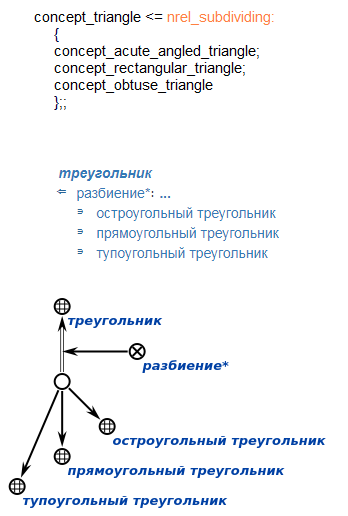
\includegraphics[width=50mm]{./part1/pictures/ostis-basics-1.png}
		\end{column}
	\end{columns}
\end{frame}

\begin{frame}{\\Информация VS знания}
	\vspace{10mm}
	Данные -- набор значений (фактов, цифр и т.д.)\\
	Пример: статистика кликов пользователя на элементы управления заданного сайта \\
	\vspace{5mm}
	Информация -- любые сведения об окружающем мире независимо от формы их представления \\
	Пример: голосовое сообщение \\
	Пример: номер телефона \\
	\vspace{5mm}
	Знания -- семантически и синтаксически целостная информация \\
	Пример: теорема Пифагора \\
	Пример: рецепт приготовления торта «Наполеон»
\end{frame}




\begin{frame}{\\Информация VS знания}
	\vspace{10mm}
	\begin{columns}[T,onlytextwidth]
		\begin{column}{0.5\textwidth}
			\vspace{20mm}
			Одна из ключевых отличительных особенностей знаний – интерпретируемость. \\
			(Дмитрий Александрович Поспелов)
		\end{column}
		\begin{column}{0.5\textwidth}
			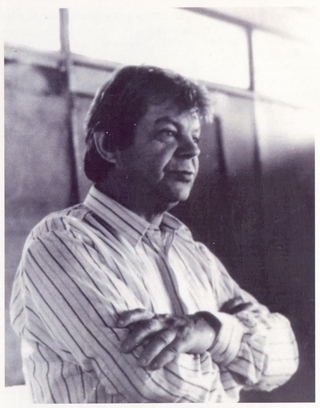
\includegraphics[width=50mm]{./part1/pictures/sc-code-pospelov.jpg}
		\end{column}
	\end{columns}
\end{frame}


\begin{frame}{\\Семантические сети}
	Семантическая сеть -- граф, вершины которого являются знаками некоторых сущностей, а дуги (ребра) – знаками связей между этими сущностями
	\\
	Семантика знака -- отношение между знаком и сущностью (значением знака, денотатом), которую он обозначает.
	\\
	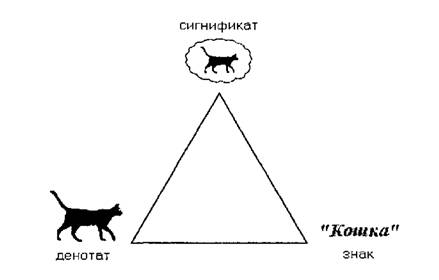
\includegraphics[width=50mm]{./part1/pictures/sc-code-cat.jpg}
\end{frame}
